% This is "sig-alternate.tex" V2.1 April 2013
% This file should be compiled with V2.5 of "sig-alternate.cls" May 2012
%
% This example file demonstrates the use of the 'sig-alternate.cls'
% V2.5 LaTeX2e document class file. It is for those submitting
% articles to ACM Conference Proceedings WHO DO NOT WISH TO
% STRICTLY ADHERE TO THE SIGS (PUBS-BOARD-ENDORSED) STYLE.
% The 'sig-alternate.cls' file will produce a similar-looking,
% albeit, 'tighter' paper resulting in, invariably, fewer pages.
%
% ----------------------------------------------------------------------------------------------------------------
% This .tex file (and associated .cls V2.5) produces:
%       1) The Permission Statement
%       2) The Conference (location) Info information
%       3) The Copyright Line with ACM data
%       4) NO page numbers
%
% as against the acm_proc_article-sp.cls file which
% DOES NOT produce 1) thru' 3) above.
%
% Using 'sig-alternate.cls' you have control, however, from within
% the source .tex file, over both the CopyrightYear
% (defaulted to 200X) and the ACM Copyright Data
% (defaulted to X-XXXXX-XX-X/XX/XX).
% e.g.
% \CopyrightYear{2007} will cause 2007 to appear in the copyright line.
% \crdata{0-12345-67-8/90/12} will cause 0-12345-67-8/90/12 to appear in the copyright line.
%
% ---------------------------------------------------------------------------------------------------------------
% This .tex source is an example which *does* use
% the .bib file (from which the .bbl file % is produced).
% REMEMBER HOWEVER: After having produced the .bbl file,
% and prior to final submission, you *NEED* to 'insert'
% your .bbl file into your source .tex file so as to provide
% ONE 'self-contained' source file.
%
% ================= IF YOU HAVE QUESTIONS =======================
% Questions regarding the SIGS styles, SIGS policies and
% procedures, Conferences etc. should be sent to
% Adrienne Griscti (griscti@acm.org)
%
% Technical questions _only_ to
% Gerald Murray (murray@hq.acm.org)
% ===============================================================
%
% For tracking purposes - this is V2.0 - May 2012

\documentclass{sig-alternate-05-2015}

\usepackage{qtree}
\newcommand{\lss}{LSS}
\begin{document}

% Copyright
\setcopyright{acmcopyright}
%\setcopyright{acmlicensed}
%\setcopyright{rightsretained}
%\setcopyright{usgov}
%\setcopyright{usgovmixed}
%\setcopyright{cagov}
%\setcopyright{cagovmixed}


% DOI
\doi{10.475/123_4} %D What goes here?

% ISBN
\isbn{123-4567-24-567/08/06}  %D What goes here?

%Conference
\conferenceinfo{PLDI '13}{June 16--19, 2013, Seattle, WA, USA}  %D What goes here?

\acmPrice{\$15.00}  %D What goes here?

%
% --- Author Metadata here ---
\conferenceinfo{WOODSTOCK}{'97 El Paso, Texas USA}  %D What goes here?
%\CopyrightYear{2007} % Allows default copyright year (20XX) to be over-ridden - IF NEED BE.
%\crdata{0-12345-67-8/90/01}  % Allows default copyright data (0-89791-88-6/97/05) to be over-ridden - IF NEED BE.
% --- End of Author Metadata ---

\title{Position Paper: A Literate Framework %D or Tool?
for Scientific Software Development
\titlenote{(Produces the permission block, and
copyright information). For use with
SIG-ALTERNATE.CLS. Supported by ACM.}}
\subtitle{[Extended Abstract]
\titlenote{A full version of this paper is available as
\textit{Author's Guide to Preparing ACM SIG Proceedings Using
\LaTeX$2_\epsilon$\ and BibTeX} at
\texttt{www.acm.org/eaddress.htm}}}

\numberofauthors{3} 
\author{
%D No idea what the ordering of this section should be
\alignauthor
Dan Szymczak\\
       \affaddr{McMaster University}\\
       \affaddr{1280 Main Street W}\\
       \affaddr{Hamilton, Ontario}\\
       \email{szymczdm@mcmaster.ca}
\alignauthor
Spencer Smith\\
       \affaddr{McMaster University}\\
       \affaddr{1280 Main Street W}\\
       \affaddr{Hamilton, Ontario}\\
       \email{smiths at mcmaster.ca} 
%D Not sure if you want your email machine-readable
\alignauthor
Jacques Carette\\
       \affaddr{McMaster University}\\
       \affaddr{1280 Main Street W}\\
       \affaddr{Hamilton, Ontario}\\
       \email{carette at mcmaster.ca}
%D Not sure if you want your email machine-readable
}
\date{24 January 2016}

\maketitle
\begin{abstract}
Awesome abstract that makes readers fall in love with the research
and throw grant money at us in droves goes here.
\end{abstract}


%
% The code below should be generated by the tool at
% http://dl.acm.org/ccs.cfm
% Please copy and paste the code instead of the example below. 
%

%TODO: THIS
\begin{CCSXML}
<ccs2012>
 <concept>
  <concept_id>10010520.10010553.10010562</concept_id>
  <concept_desc>Computer systems organization~Embedded systems</concept_desc>
  <concept_significance>500</concept_significance>
 </concept>
 <concept>
  <concept_id>10010520.10010575.10010755</concept_id>
  <concept_desc>Computer systems organization~Redundancy</concept_desc>
  <concept_significance>300</concept_significance>
 </concept>
 <concept>
  <concept_id>10010520.10010553.10010554</concept_id>
  <concept_desc>Computer systems organization~Robotics</concept_desc>
  <concept_significance>100</concept_significance>
 </concept>
 <concept>
  <concept_id>10003033.10003083.10003095</concept_id>
  <concept_desc>Networks~Network reliability</concept_desc>
  <concept_significance>100</concept_significance>
 </concept>
</ccs2012>  
\end{CCSXML}

\ccsdesc[500]{Computer systems organization~Embedded systems}
\ccsdesc[300]{Computer systems organization~Redundancy}
\ccsdesc{Computer systems organization~Robotics}
\ccsdesc[100]{Networks~Network reliability}


%
% End generated code
%

%
%  Use this command to print the description
%
\printccsdesc

\keywords{ACM proceedings; \LaTeX; text tagging}

\section{Introduction}
Scientific computing (SC) was the first application of computers. It is still
used today for a wide variety of tasks: constructing mathematical models,
performing quantitative analyses, creating simulations, solving scientific
problems, etc. SC software has been developed for increasingly safety and
security critical systems (nuclear reactor simulation, satellite
guidance%D MORE EXAMPLES)
) as well as predictive
systems.
It has applications including (but not limited to) predicting weather patterns
and natural disasters, and simulating economic fluctuations. As such, it is an
incredibly important part of an increasing number of industries
today.

In the medical, nuclear power, aerospace, automotive, and manufacturing fields
there are many safety critical systems in play. With each system, there is the
possibility of a catastrophic failure endangering lives. It is incredibly
important then to have some means of certifying and assuring the quality of each
software system. As Smith et al. \cite{SmithEtAl2013} stated
``Certification of Scientific Computing (SC) software is official recognition by
an authority or regulatory body that the software is fit for its intended use.''
These regulatory bodies determine certain certification standards that must be
met for a system to become recognized as certified. One example of a
certification standard is the Canadian Standards Association (CSA) requirements
for quality assurance of scientific software for nuclear power plants.

The main goal of software certification is to ``... systematically determine,
based on the principles of science, engineering, and measurement theory, whether
a software product satisfies accepted, well-defined and measurable criteria''
\cite{HHLMWW}. As such, certification would not only involve analyzing the code
systematically and rigorously, but also analyzing the
documentation. Essentially, this means the software must be both valid and
verifiable, reliable, usable, maintainable, reusable, understandable, and
reproducible. %D Verification involves ensuring that the software is ``solving
              %the equations right'', whereas validation requires ensuring that
              %the software is ``solving the right equations''\cite{Roache1998}.

Developing certifiable software can end up being a much more involved process
than developing uncertified software: it takes more money, time, and effort on
the part of developers to produce. These increased costs lead to reluctance from
practitioners to develop certifiable software \cite{Roache1998}. However, in
our 
opinion, cost is not the only contributing factor for the developers. As it
stands in the field, scientists seem to prefer a more agile development process
\cite{Segal2008}. However, this is not necessarily the best process as typically
this would lead to problems maintaining the
documentation, meaning that not all aspects of the software would be traceable
through the design process and making certification more difficult (if not
impossible).

Given proper methods and tools, scientists would be able to follow a more
structured approach (while capitalizing on frequent feedback and course
correction) to meet documentation requirements for certification as well as
improve their overall productivity. This is where our work comes in: our goal is
to eat our cake and have it too.  We want to improve the qualities
(verifiability, reliability, understandability etc.) of SC software and at the
same time
improve performance.  Moreover, we want to improve developer productivity; save
time and money on SC software development, certification and
re-certification. To accomplish this we need to do the following:

\begin{enumerate}
\item Remove duplication between software artifacts for SC
  software \cite{WilsonEtAl2013}
\item Provide complete traceability between all software artifacts
\end{enumerate}

%D Introduce artifacts somewhere?

To achieve the above goals, we propose the following:

\begin{enumerate}
\item Provide methods, tools and techniques to support developing scientific
  software using a literate process
\item Automate software artifact generation
\end{enumerate}

Section~\ref{sec:background} will give a more in-depth look at SC software,
specifically focusing on SC software quality and literate programming. 
Section~\ref{sec:lss} focuses on our framework %D Tool?
for improving SC software development using a structured approach. It will
introduce the framework, discuss the advantages to our approach, and show
a short example of the framework in action. Section~\ref{sec:todo} will discuss
how we want the framework to evolve and what future work we intend to do.
Finally, Section~\ref{sec:conclusion} will provide some concluding remarks.

%Context
%- first application of computers was scientific computing (SC)
%- the importance of SC code - used for decisions that impact health, safety and the economy
%- important enough to follow certification standards in some cases, CSA, Roache
%- problem with standards is the time and money required to meet them, resistance from practitioners (can cite Roache to support this)
%- many scientists seem to prefer a more agile development process (cite Carver, Kelly and Segal - see Smith book chapter for specific references), but this does not mean that this is the best process - with the proper methods and tools, scientists can follow a more structured approach, and still focus on frequent feedback and course correction - can meet documentation requirements for certification, and improve productivity.
%
%Our goal is to have our cake and eat it too.  We want to improve the qualities (verifiability, reliability, understandability etc.) especially traceability.  Moreover, we want to improve productivity. Save time and money on SC software development, certification and re-certification.  Improving traceability also allows us to improve reproducibility (cite Davison2012) because the decisions and details are explicitly available in the future.
%
%To accomplish this we need to do the following:
%
%- Remove duplication between software artifacts for scientific computing software (can cite Wilson et al DRY principle)
%- Provide a means for complete traceability between all artifacts
%
%To achieve the above two goals, we propose the following:
%
%- Provide tools to support developing scientific software using a literate process
%- Use artifact generation
%
%- roadmap of the sections that are coming

\section{Background} \label{sec:background}

Throughout the history of computing, specifically scientific computing, there
have been many challenges towards assuring the quality of software. Many
attempts have been made (some successful, others not) at improving software
quality. In this section we will discuss those challenges, as well
as introduce the ideas behind our proposed approach.

\subsection{Challenges for Scientific Computing Software Quality} \label{ssec:challenges}

SC software has certain characteristics which create challenges for its
development. We will not discuss them all in depth, however, those of interest
to us are the technique selection, input output (or understandability), and
modification (or maintainability) challenges as described by Yu \cite{Yu2011}.

The \textit{technique selection challenge} is a challenge that comes up often
when dealing with continuous mathematical equations. Since these cannot be
solved directly (due to computers being discrete), some technique must be chosen
which can produce a solution which is ``good enough'' for the user. Choosing the
technique to use is typically left to domain experts as each technique will
(not) satisfy certain non-functional requirements.

The \textit{understandability} challenge impacts the usability of SC software and
typically comes up where considerable amounts of input data are used in the
production of large volumes of output. The main issue in this case is the
complicated nature of the input data and the output, leading developers to
recreate existing library routines (slightly modified) to deal with the
nature of the input and output. Programmers do not reuse libraries as often as they could because they do not believe that the interface needs to be as complicated as it appears \cite{Dubois2002}.

Finally, the \textit{maintainability challenge} tends to come up as requirements
change. As SC software is used at the forefront of scientific knowledge, there
can be a high frequency of requirements changes. As changing requirements can
mean completely modified systems, it poses a problem for scientists: commercial
software can be difficult/expensive to modify and noncommercial programs are not
often flexible enough to change.

%From Yu (2011) (PhD thesis, now in our repository)
%- technique selection challenge - [I think we can keep this challenge, if we later mention how LSS encourages a separation of concerns between requirements (model) and design (numerical algorithm selection).  LSS also allows for experimentation with different numerical techniques.]  
%- input output challenge [I think we should keep this one, but we should characterize it as an understandability challenge.  Programmers do not reuse libraries as often as they could because they do not believe that the interface needs to be as complicated as it appears (Dubois2002).  We can mention this challenge again later, because LSS will allow us to create programs, and interfaces, that are only as complicated as they need to be.]
%- modification challenge [I think we could relabel this as a maintainability challenge.]

\subsection{Literate Programming} \label{ssec:literate}

Literate programming (LP) is a programming methodology introduced by Knuth
\cite{Knuth1984}. The main idea behind it is writing programs in a way that
allows us to explain (to humans) what we want the computer to do, as opposed to
simply telling the computer what to do. There is a focus on ordering the
material to promote better human understanding.

In a literate program, the documentation and code are kept together in one
source. The program is an interconnected web of code pieces, presented in any
sequence. As part of the development process, the algorithms used in literate
programming are broken down into small, easy to understand parts (known as
``sections'' \cite{Knuth1984} or ``chunks'' \cite{Johnson1997}) which are
explained, documented, and implemented in a more intuitive order for better
understanding.

To extract the source code or documentation from the literate program,
certain processes must be run. To get working source code, the \textit{tangle}
process would be run, essentially extracting the code from the literate document
and reordering it into an appropriate structure for the computer to
understand.  To get a human-readable document, the \textit{weaving}
process must be run to extract and typeset the documentation.

By adhering to the LP methodology, a literate program ends up with documentation
that is expertly written and of publishable quality. The code also ends up being
incredibly well documented and high-quality. There are several examples of SC
programs being written in LP style, and two that stand out are VNODE-LP
\cite{Nedialkov2006} and ``Physically Based Rendering: From Theory to
Implementation'' \cite{PharrAndHumphreys2004} (a literate program which is also
a full textbook).

\section{Introducing \lss} \label{sec:lss} % (NEED A BETTER NAME)

Our framework, \lss, is being developed with the goals of providing complete
traceability throughout the development process for SC software and reducing
the amount of knowledge duplication across software artifacts. Both of these
goals can be accomplished by following a (somewhat modified) literate approach.

The current framework is composed of several components including 
\textit{chunks}, \textit{recipes}, and a \textit{generator}.
The generator produces views of the source material, where these views are
the software artifacts we require. Recipes are essentially descriptions
of these views and chunks contain the source material.

Complete traceability is achievable through the use of chunks,
providing that all requisite knowledge can be appropriately encapsulated.
Each chunk needs to represent some concept, quantity, unit, etc. Our current design introduces a chunk hierarchy 
(as seen in Figure~\ref{fig:chunks}), where the most basic
chunk has only one field: a \textit{name}. A ``Concept'' then adds a 
\textit{description}, and so on down the tree.

\begin{figure}
\large{
\Tree[.\fbox{Chunk(\textit{name})}
		[.\fbox{Concept(\textit{description})}
			[.\fbox{Quantity(\textit{symbol})} ]
			[.\fbox{Unit(\textit{unit})} ]
		]
	]
}
\caption{The chunk hierarchy design}
\label{fig:chunks}
\end{figure}

Each more complex chunk is built from one or more of the existing chunks.
This will be shown in more detail through the example in 
Section~\ref{ssec:example}.
%D Maybe introduce the example here for clarity?
Thus, all of the information related to any one
concept in a software project will be stored in a single chunk, allowing
for complete traceability to the source of the information.

Recipes are specified using a micro- and macro-layout language currently
embedded in Haskell. Each are used to describe how the generated artifacts
should appear. The micro-layout language handles the small-scale layout 
details such as those of specially
formatted characters (i.e. subscript and superscripts), concatenation of
symbols, etc. The macro-layout language, on the other hand, handles the
large-scale layout details such as sections, paragraphs, equations, 
tables, etc.

Recipes also specify which knowledge should be used from which chunks, thus
removing knowledge duplication as all of the knowledge is now being referenced
from within the specified chunks.

%- Tie the introduction of the paper into the tool.
%- Introduce the ideas of recipes and chunks.
%- Explain some of the current design?
%  - i.e. Chunk hierarchy diagram, recipe micro/macro layout languages, code gen

\subsection{Advantages} \label{ssec:advantages}

- Move into examples/discussion on advantages. Should write something here.

\subsubsection{Software Certification} \label{sssec:adv_cert}
%- need to generate required documentation, without impeding the work of the scientists
%- need to be able to make changes at reasonable cost - this requires traceability

%- Discuss the following documents as being "par for the course" but maybe don't 
%  include full descriptions:
%    Start with a default set of documentation, as follows
%    - Problem Statement
%    - Development Plan
%    - Requirements Specification
%    - Verification and Validation plan
%    - Design Specification
%    - Code
%    - Verification and Validation Report
%    - User Manual

To certify software there is a need for high-quality documentation. This
documentation needs to be created without impeding the work of scientists. One
of the major problems with creating documentation for SC software stems from the
maintainability challenge (Section~\ref{ssec:challenges}). As the requirements
change, the documentation must be updated. The further scientists are into a
project, the greater the effect a change in requirements will have on the
documentation, leading to maintainability and traceability issues.

The cost of making changes to the documentation should be reasonable. The best
way to keep costs low is to ensure the traceability of the documentation.
Traceability allows the developers to track which areas of a project will be
affected by a change, thus allowing them to ensure that those areas are updated
accordingly.

Depending on the regulatory body and set of standards for certification, many
types of documents can be required. \lss aims to generate all of these documents
alongside the code, while accounting for any changes made. As the changes will
affect chunks and those chunks will be used to generate the documentation and
code, there is a guarantee that changes will propagate throughout all of the
artifacts. The following are examples software artifacts that we wish to
generate (we assume software engineers will be familiar with most, if not all,
of these):

\begin{enumerate}
\item Problem Statement
%  A description of the problem to be solved, essentially
%  summarizing the purpose of the software. There should be no mention of how the
%  problem is to be solved.
\item Development Plan
%  An overview of the development process and
%  infrastructure. This should cover the documents to be created, which templates
%  (if any) will be followed, internal processes to be employed, coding
%  standards, and other details relevant to how the software will be developed.
\item Requirements Specification
%  The desired functions and qualities of the
%  software should be documented herein. The requirements should cover
%  functionality, goals, context, design constraints, expected performance, and
%  any other quality attributes of the software.
\item Verification and Validation plan
%  Documents how the documentation
%  artifacts will be shown to be internally correct (verification) as well as how
%  to ensure that the right problem has been solved (validation).
\item Design Specification
%  How will the requirements be realized? Document the
%  software architecture and a detailed design of the modules/interfaces to be
%  used. Can be thought of as a programmer's manual for maintenance.
\item Code
%  Implementation of the design specification.
\item Verification and Validation Report
%  Summarize the steps taken for
%  performing verification and validation (this should mirror the V \& V plan
%  from above) and include any testing results.
\item User Manual
%  Full instructions on how the software is to be used,
%  beginning with installation instructions and proceeding through detailed
%  examples of the program's use.
\end{enumerate}

The artifacts listed above share non-trivial amounts of information, which is
where traceability comes into play. To make any changes to the
documentation, there must be some way to determine how a change will affect
\textbf{all} of the documents.

This is especially important for (re-) certification, as the documents must be 
consistent.

In the context of re-certification, if a piece of software was developed using
\lss and some changes needed to be made, updating the artifacts and submitting
them for re-certification would be completely trivial. All documentation would
be generated from the (newly modified) chunks, according to their existing
recipes. Or in the case of new information being added, a new chunk would be
created and the recipe slightly modified.

On another note, if a document standard were to be changed during the 
development cycle, it would not necessitate re-writing the entire document. All
of the information in the chunks would remain intact, only the recipe 
would need to be changed to accomodate the new standard.

\subsubsection{Knowledge Capture} \label{sssec:adv_knowledge}

In SC software there are many commonly shared theorems and formulae between
different applications. For an example consider the conservation of thermal
energy equation: 
\begin{displaymath} 
-{\bf \nabla q} + g = \rho C \frac{\partial T}{\partial t}
\end{displaymath} 
This
equation is widely used in a variety of thermal analysis applications, where
each is solving a different problem, or modeling a different system.

Our approach aims to build libraries of chunks that can be reused in many
different applications. Each library should contain common chunks relevant to a
specific application domain (ex. thermal analysis) and each project should aim
to reuse as much as possible during development.

A more abstract, yet more common example of a reused knowledge source is the
concept of Syst\'{e}me International (SI) units. They are used in applications
throughout all of SC, so why should they be redefined for each project? Once the
knowledge has been captured, they can simply be reused wherever necessary.

\subsubsection{"Everything should be made as simple as possible, but not simpler."  (Einstein quote)} \label{sssec:adv_simple}

Currently there exist many powerful, general commercial programs for solving
problems using the finite element method. However, they are not often used
to develop new ``widgets'' because of the cost and complexity of doing so.
As it stands, engineers often have to resort to building prototypes and testing
them instead of performing simulations due to a lack of tools that can assist
with their exact set of problems.

Our approach could change that by generating source code suited to the needs of
the engineers. For example, if an engineer were designing parts for strength,
the could have a general stress analysis program. This program could be 3D or
specialized for plane stress or strain, depending on which assumption would be
most appropriate. The program could even be customized to the parameterized
shape of the part that the engineer is interested in. The new program would also
only expose the degrees of freedom necessary for the engineer to change (ex.
material properties or specific dimensions of the part), making the simulation
process simpler and safer.

\lss will tackle the understandability challenge (Section~\ref{ssec:challenges})
by allowing developers to build components which will provide exactly what is
needed, no more and no less.

\subsubsection{Verification} \label{sssec:adv_verify}

- requirements include so-called “sanity” checks that can be reused when they come up in subsequent phases
- for instance, requirement would state conservation of mass, or the fact that lengths are always positive - the first used to test output, the second to guard against invalid input

- computational variability testing, from Yu (2011), FEM example
- usual to do grid refinement tests - same order of interpolation, but more points
- code generation allows for increases in the order of interpolation, for the same grid
- Yu discusses in section 6.3 of her thesis

\subsubsection{Testing} \label{sssec:adv_test}% Maybe move this to future work?

- ???

\subsection{Bringing it together with an example} \label{ssec:example}

- Introduce fuel pin example.
- Use appendix for SRS and generated SRS?

\subsubsection{How it works} \label{sssec:ex_how}
- Explain the source (recipe, common knowledge, specific knowledge)
- Show example recipe
- Example of common knowledge (SI Units to tie into section 3.1.2)
- Example of specific knowledge ($h_c$ or $h_g$ chunk)

\subsubsection{The result?} \label{sssec:ex_result}

- Bring it all back to the arguments made in 3.1.1-3.1.4 and justify them.

- 3.1.1: (Ideally) No cost to make changes, no longer impedes the scientists.
    - Explain in-depth

- 3.1.2: SI Units shows that common knowledge is easily stored to be used elsewhere
    - No need to reinvent the wheel! Keeps things consistent across projects.
    
- 3.1.3: (Ideally) Prototyping becomes trivial due to code gen.
    - Any changes to spec can be seen in (essentially) real-time.
    
- 3.1.4: Any mistakes that occur in the software artifacts occur everywhere.
    - Easier to find errors since they propagate through all the artifacts.
    - Documents are never out of sync with the source.

\section{Future work} \label{sec:todo}

- Generate more document types (more default recipes)
- Include more types of information in chunks (PCM SRS example of constraints, etc.)
  - Auto-generate test cases! Use constraint/typical value info to create tests.
  - Use constraints for errors and typical values for warnings.
- Expand the tool practically through examples.
    
\section{Concluding Remarks} \label{sec:conclusion}

%\section{The {\secit Body} of The Paper}

%\subsection{Type Changes and {\subsecit Special} Characters}
%We have already seen several typeface changes in this sample.  You
%can indicate italicized words or phrases in your text with
%the command \texttt{{\char'134}textit}; emboldening with the
%command \texttt{{\char'134}textbf}
%and typewriter-style (for instance, for computer code) with
%\texttt{{\char'134}texttt}.  But remember, you do not
%have to indicate typestyle changes when such changes are
%part of the \textit{structural} elements of your
%article; for instance, the heading of this subsection will
%be in a sans serif\footnote{A third footnote, here.
%Let's make this a rather short one to
%see how it looks.} typeface, but that is handled by the
%document class file. Take care with the use
%of\footnote{A fourth, and last, footnote.}
%the curly braces in typeface changes; they mark
%the beginning and end of
%the text that is to be in the different typeface.
%
%You can use whatever symbols, accented characters, or
%non-English characters you need anywhere in your document;
%you can find a complete list of what is
%available in the \textit{\LaTeX\
%User's Guide}\cite{Lamport:LaTeX}.

%\subsection{Math Equations}

%\subsubsection{Inline (In-text) Equations}
%A formula that appears in the running text is called an
%inline or in-text formula.  It is produced by the
%\textbf{math} environment, which can be
%invoked with the usual \texttt{{\char'134}begin. . .{\char'134}end}
%construction or with the short form \texttt{\$. . .\$}. You
%can use any of the symbols and structures,
%from $\alpha$ to $\omega$, available in
%\LaTeX\cite{Lamport:LaTeX}; this section will simply show a
%few examples of in-text equations in context. Notice how
%this equation: \begin{math}\lim_{n\rightarrow \infty}x=0\end{math},
%set here in in-line math style, looks slightly different when
%set in display style.  (See next section).

%\subsubsection{Display Equations}
%A numbered display equation -- one set off by vertical space
%from the text and centered horizontally -- is produced
%by the \textbf{equation} environment. An unnumbered display
%equation is produced by the \textbf{displaymath} environment.
%
%Again, in either environment, you can use any of the symbols
%and structures available in \LaTeX; this section will just
%give a couple of examples of display equations in context.
%First, consider the equation, shown as an inline equation above:
%\begin{equation}\lim_{n\rightarrow \infty}x=0\end{equation}
%Notice how it is formatted somewhat differently in
%the \textbf{displaymath}
%environment.  Now, we'll enter an unnumbered equation:
%\begin{displaymath}\sum_{i=0}^{\infty} x + 1\end{displaymath}
%and follow it with another numbered equation:
%\begin{equation}\sum_{i=0}^{\infty}x_i=\int_{0}^{\pi+2} f\end{equation}
%just to demonstrate \LaTeX's able handling of numbering.

%\subsection{Citations}
%Citations to articles \cite{bowman:reasoning,
%clark:pct, braams:babel, herlihy:methodology},
%conference proceedings \cite{clark:pct} or
%books \cite{salas:calculus, Lamport:LaTeX} listed
%in the Bibliography section of your
%article will occur throughout the text of your article.
%You should use BibTeX to automatically produce this bibliography;
%you simply need to insert one of several citation commands with
%a key of the item cited in the proper location in
%the \texttt{.tex} file \cite{Lamport:LaTeX}.
%The key is a short reference you invent to uniquely
%identify each work; in this sample document, the key is
%the first author's surname and a
%word from the title.  This identifying key is included
%with each item in the \texttt{.bib} file for your article.
%
%The details of the construction of the \texttt{.bib} file
%are beyond the scope of this sample document, but more
%information can be found in the \textit{Author's Guide},
%and exhaustive details in the \textit{\LaTeX\ User's
%Guide}\cite{Lamport:LaTeX}.
%
%This article shows only the plainest form
%of the citation command, using \texttt{{\char'134}cite}.
%This is what is stipulated in the SIGS style specifications.
%No other citation format is endorsed or supported.
%
%\subsection{Tables}
%Because tables cannot be split across pages, the best
%placement for them is typically the top of the page
%nearest their initial cite.  To
%ensure this proper ``floating'' placement of tables, use the
%environment \textbf{table} to enclose the table's contents and
%the table caption.  The contents of the table itself must go
%in the \textbf{tabular} environment, to
%be aligned properly in rows and columns, with the desired
%horizontal and vertical rules.  Again, detailed instructions
%on \textbf{tabular} material
%is found in the \textit{\LaTeX\ User's Guide}.
%
%Immediately following this sentence is the point at which
%Table 1 is included in the input file; compare the
%placement of the table here with the table in the printed
%dvi output of this document.
%
%\begin{table}
%\centering
%\caption{Frequency of Special Characters}
%\begin{tabular}{|c|c|l|} \hline
%Non-English or Math&Frequency&Comments\\ \hline
%\O & 1 in 1,000& For Swedish names\\ \hline
%$\pi$ & 1 in 5& Common in math\\ \hline
%\$ & 4 in 5 & Used in business\\ \hline
%$\Psi^2_1$ & 1 in 40,000& Unexplained usage\\
%\hline\end{tabular}
%\end{table}
%
%To set a wider table, which takes up the whole width of
%the page's live area, use the environment
%\textbf{table*} to enclose the table's contents and
%the table caption.  As with a single-column table, this wide
%table will ``float" to a location deemed more desirable.
%Immediately following this sentence is the point at which
%Table 2 is included in the input file; again, it is
%instructive to compare the placement of the
%table here with the table in the printed dvi
%output of this document.
%
%
%\begin{table*}
%\centering
%\caption{Some Typical Commands}
%\begin{tabular}{|c|c|l|} \hline
%Command&A Number&Comments\\ \hline
%\texttt{{\char'134}alignauthor} & 100& Author alignment\\ \hline
%\texttt{{\char'134}numberofauthors}& 200& Author enumeration\\ \hline
%\texttt{{\char'134}table}& 300 & For tables\\ \hline
%\texttt{{\char'134}table*}& 400& For wider tables\\ \hline\end{tabular}
%\end{table*}
%% end the environment with {table*}, NOTE not {table}!
%
%\subsection{Figures}
%Like tables, figures cannot be split across pages; the
%best placement for them
%is typically the top or the bottom of the page nearest
%their initial cite.  To ensure this proper ``floating'' placement
%of figures, use the environment
%\textbf{figure} to enclose the figure and its caption.
%
%This sample document contains examples of \textbf{.eps} files to be
%displayable with \LaTeX.  If you work with pdf\LaTeX, use files in the
%\textbf{.pdf} format.  Note that most modern \TeX\ system will convert
%\textbf{.eps} to \textbf{.pdf} for you on the fly.  More details on
%each of these is found in the \textit{Author's Guide}.
%
%\begin{figure}
%\centering
%%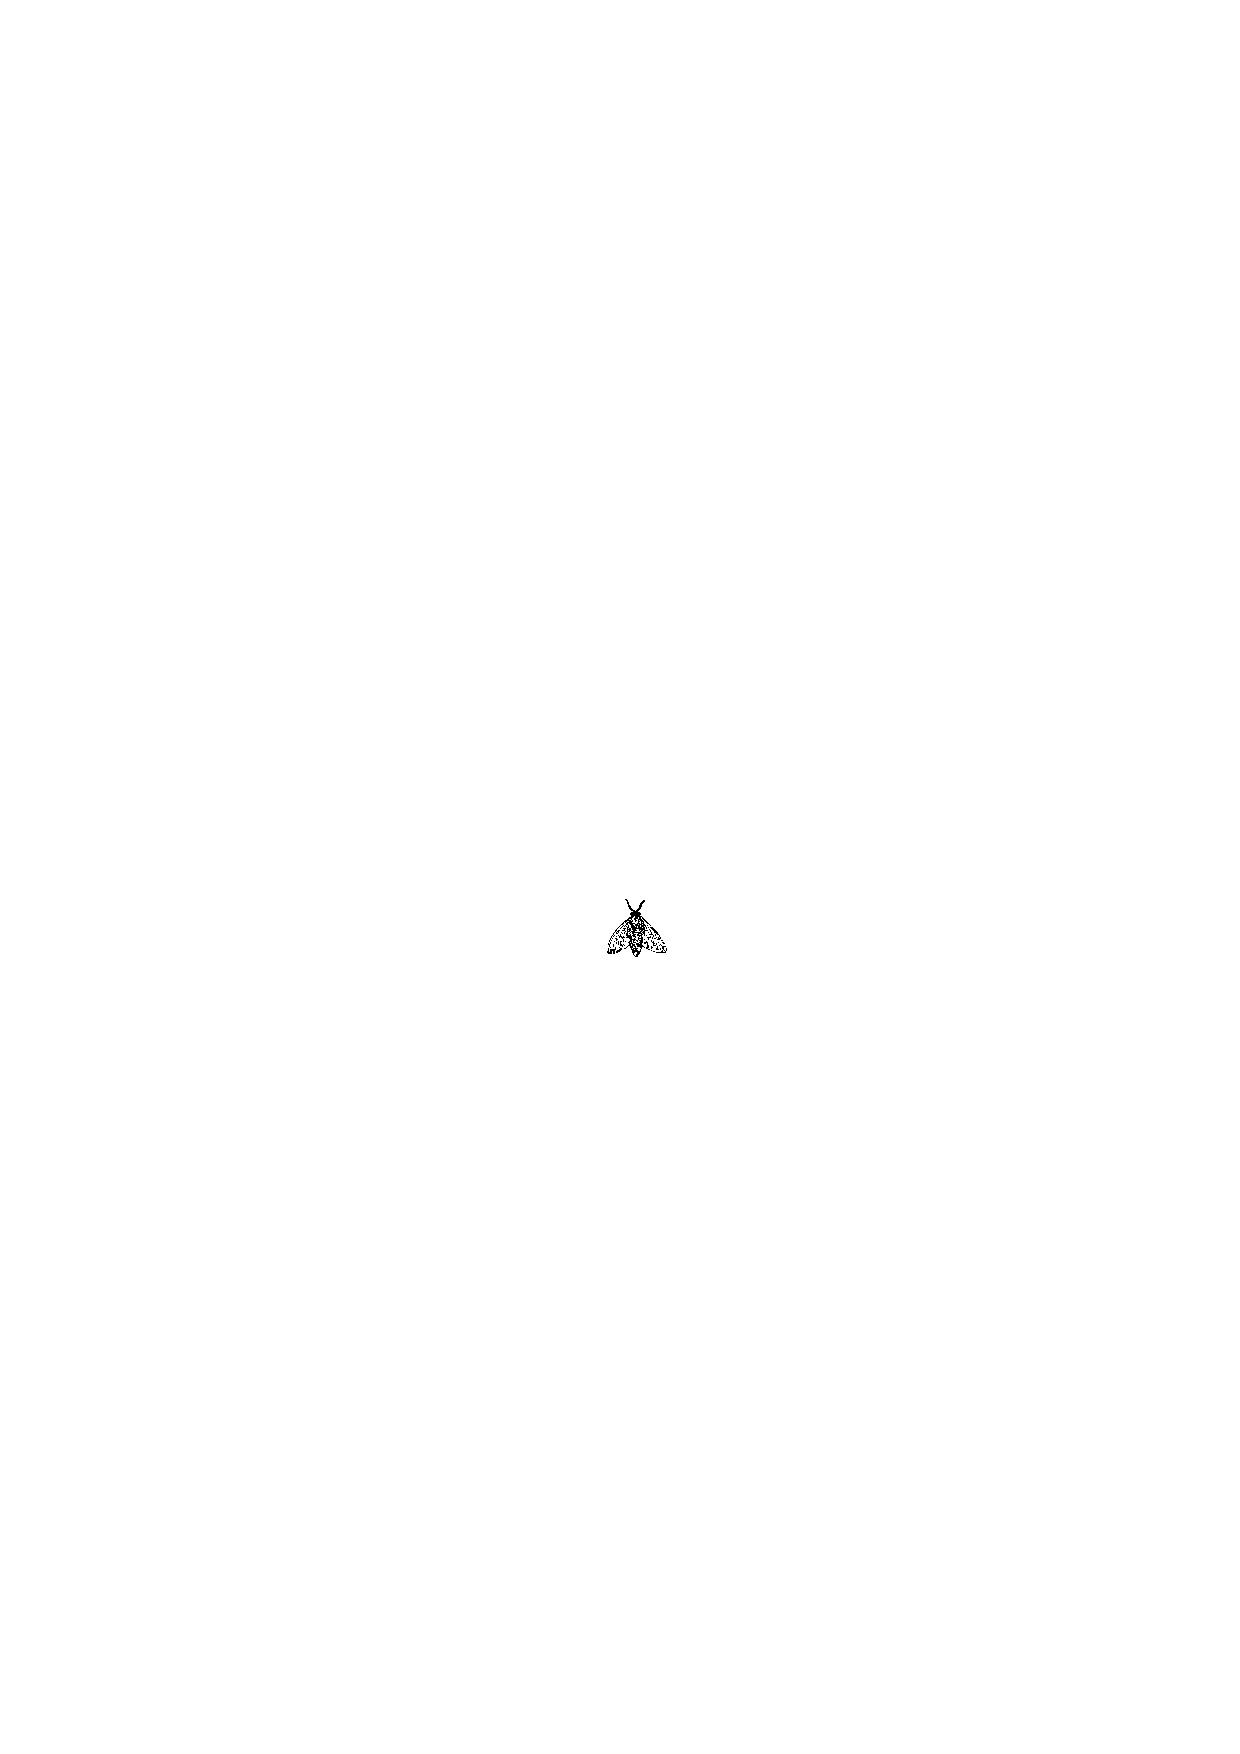
\includegraphics{fly}
%\caption{A sample black and white graphic.}
%\end{figure}
%
%\begin{figure}
%\centering
%%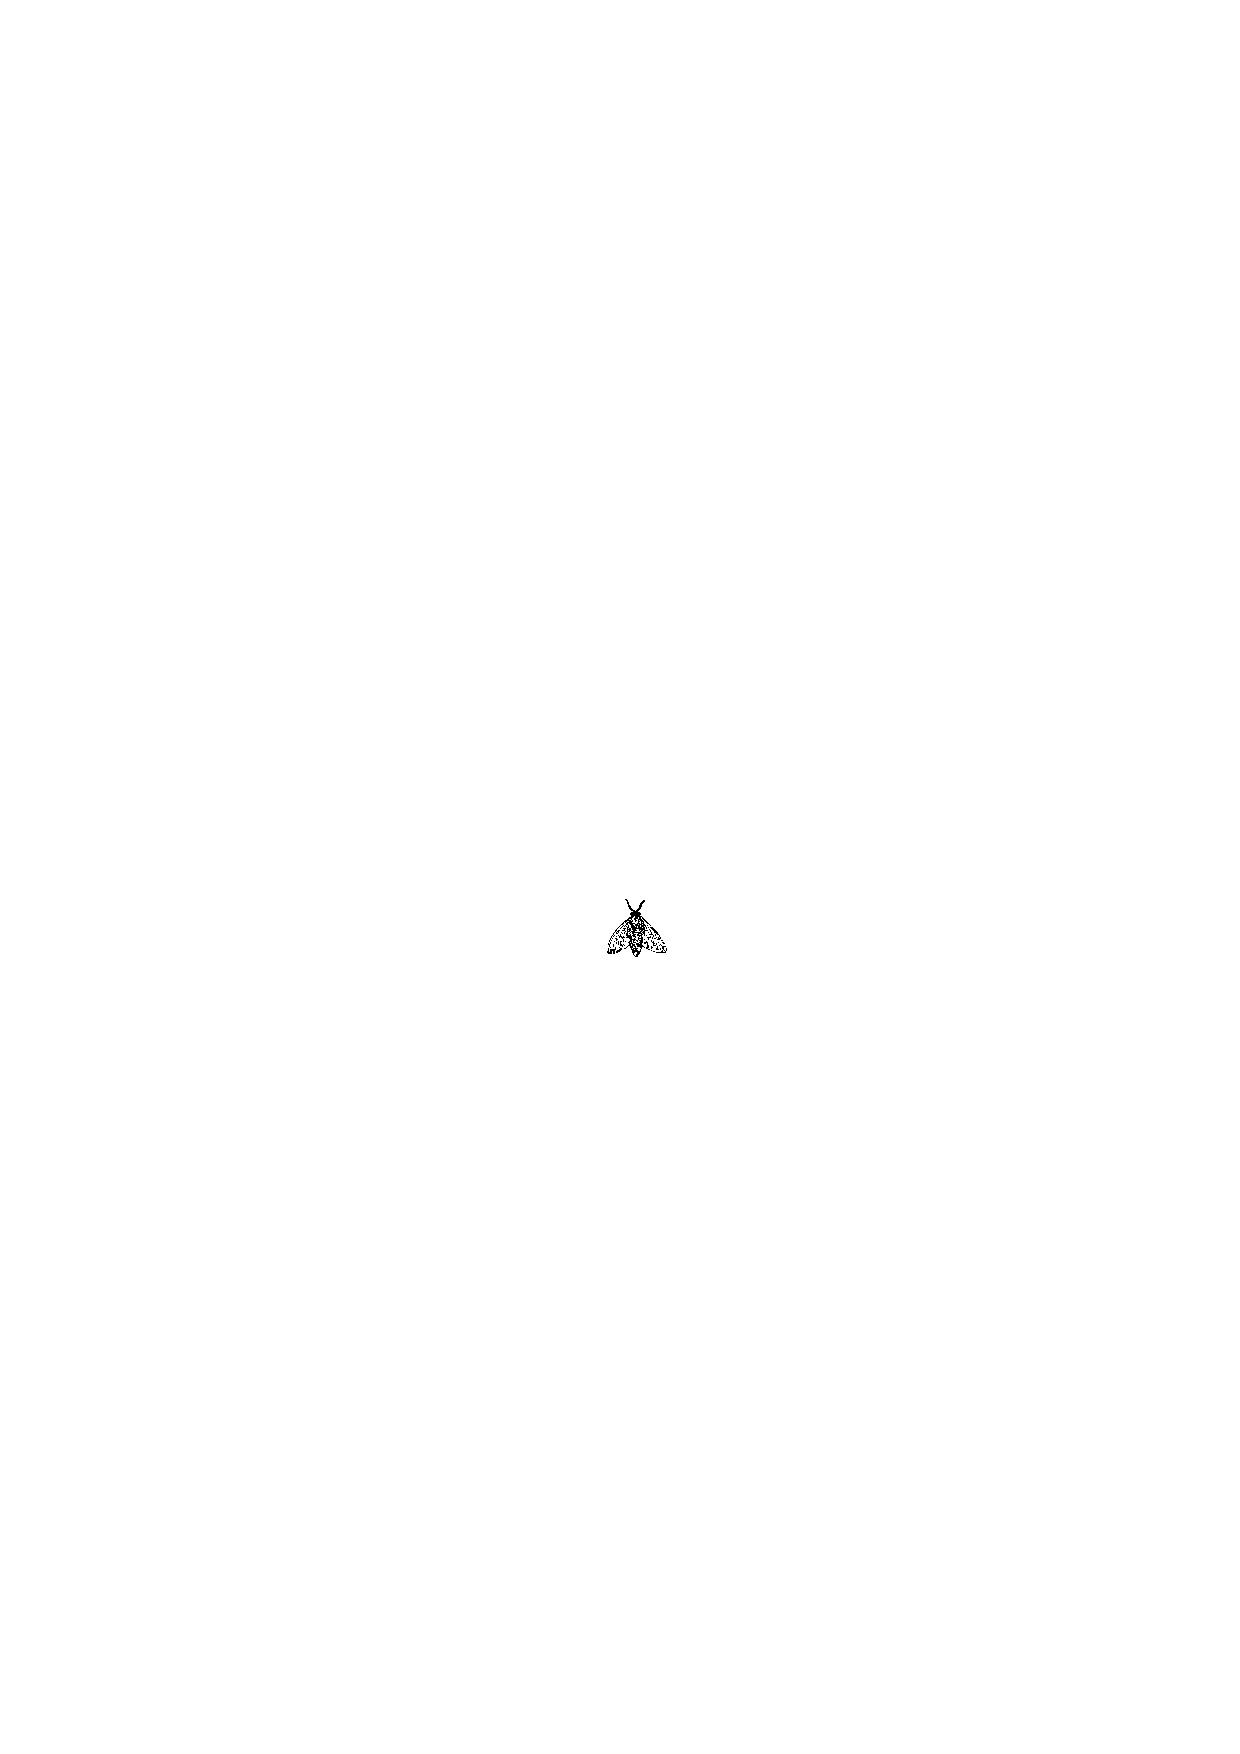
\includegraphics[height=1in, width=1in]{fly}
%\caption{A sample black and white graphic
%that has been resized with the \texttt{includegraphics} command.}
%\end{figure}
%
%
%As was the case with tables, you may want a figure
%that spans two columns.  To do this, and still to
%ensure proper ``floating'' placement of tables, use the environment
%\textbf{figure*} to enclose the figure and its caption.
%and don't forget to end the environment with
%{figure*}, not {figure}!
%
%\begin{figure*}
%\centering
%%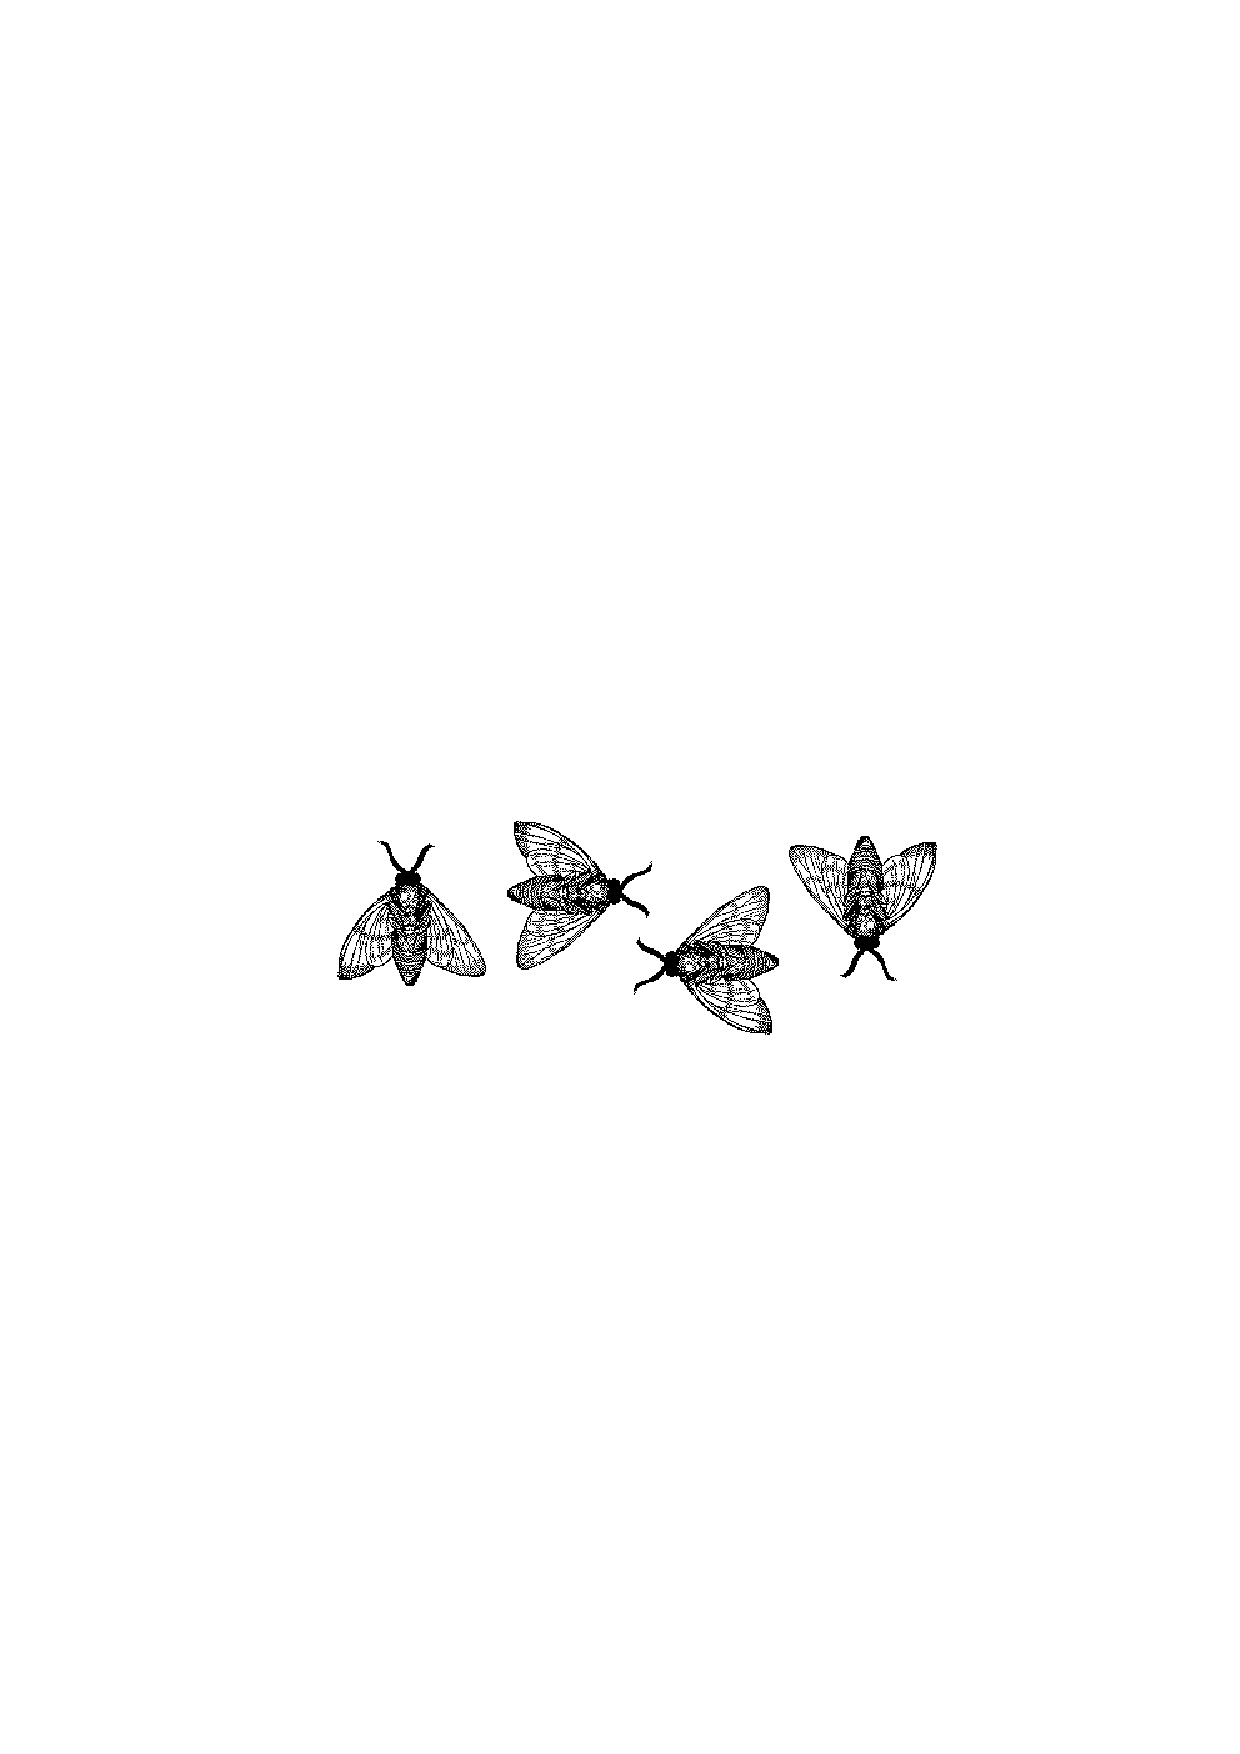
\includegraphics{flies}
%\caption{A sample black and white graphic
%that needs to span two columns of text.}
%\end{figure*}
%
%
%\begin{figure}
%\centering
%%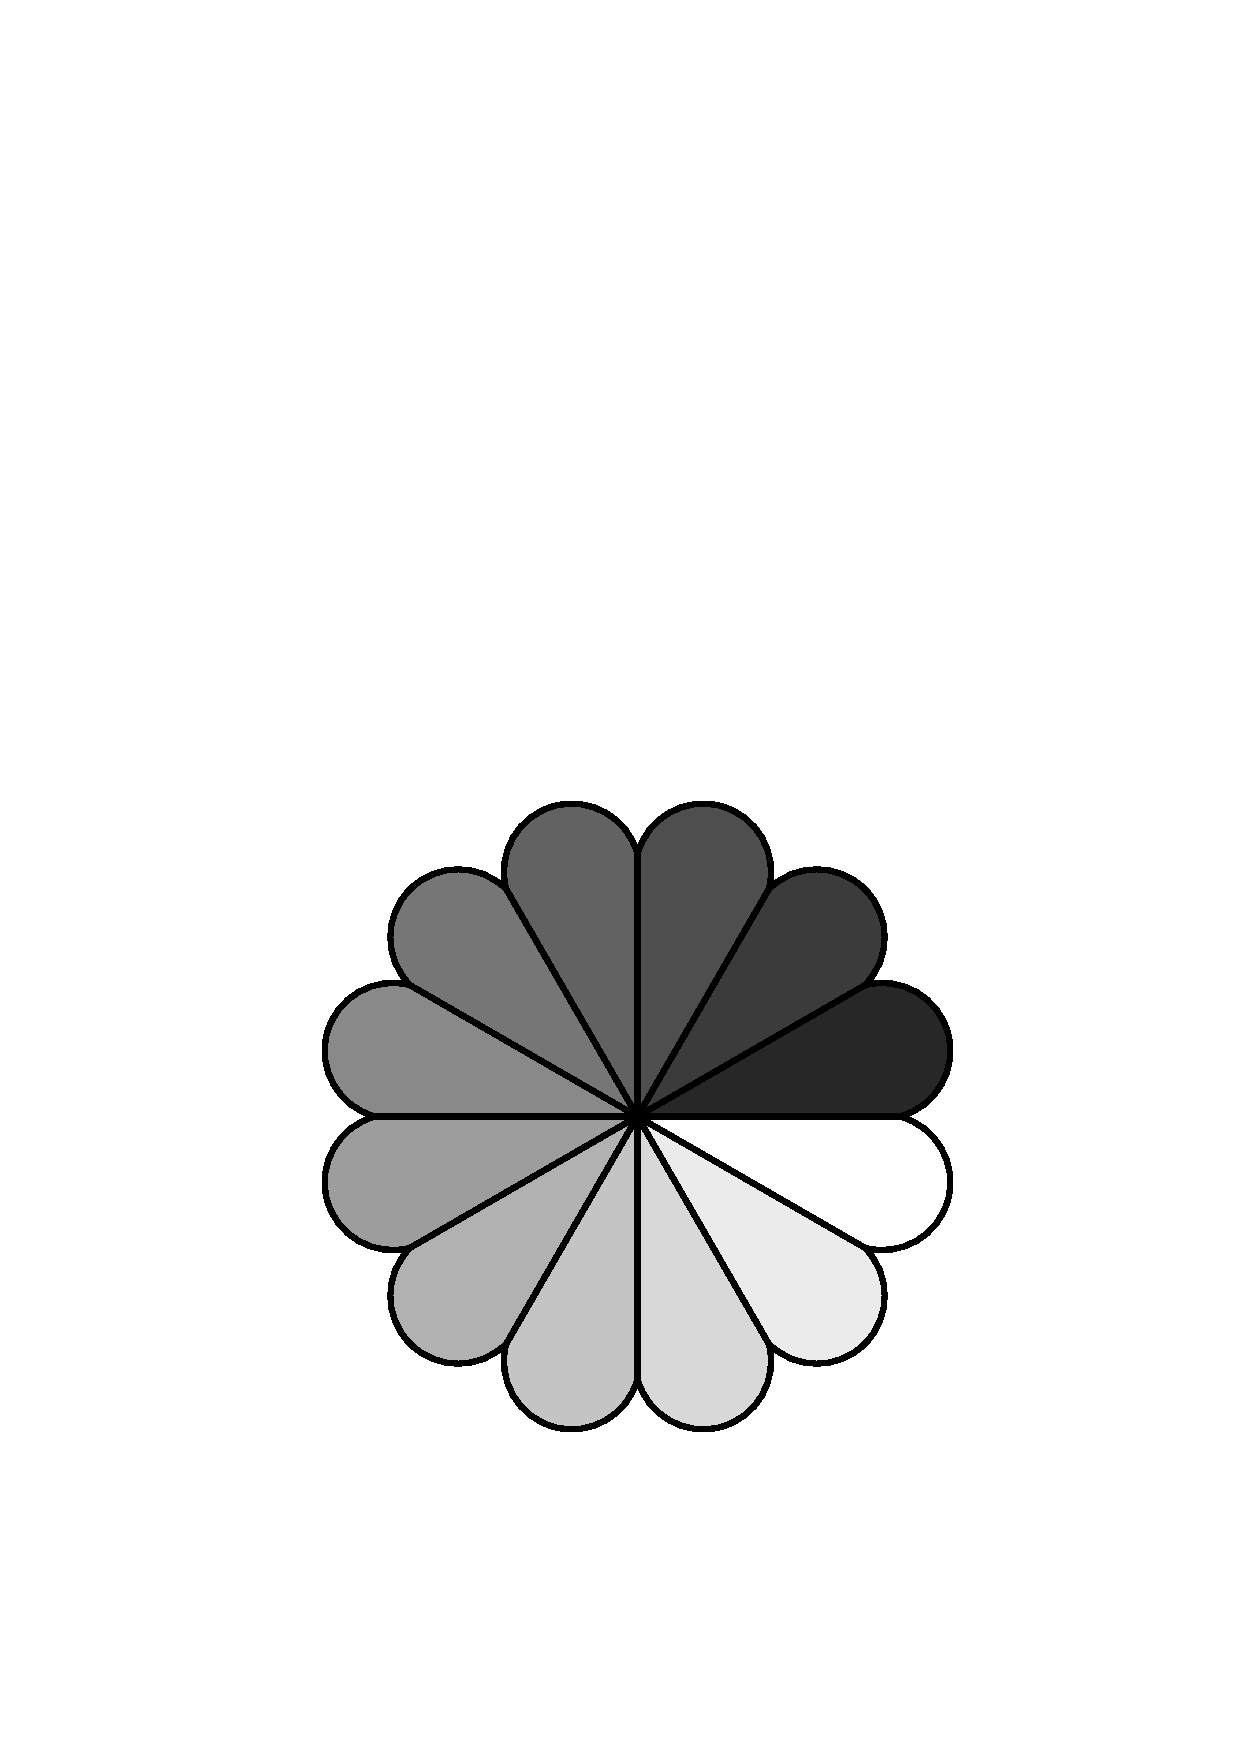
\includegraphics[height=1in, width=1in]{rosette}
%\caption{A sample black and white graphic that has
%been resized with the \texttt{includegraphics} command.}
%\vskip -6pt
%\end{figure}
%
%\subsection{Theorem-like Constructs}
%Other common constructs that may occur in your article are
%the forms for logical constructs like theorems, axioms,
%corollaries and proofs.  There are
%two forms, one produced by the
%command \texttt{{\char'134}newtheorem} and the
%other by the command \texttt{{\char'134}newdef}; perhaps
%the clearest and easiest way to distinguish them is
%to compare the two in the output of this sample document:
%
%This uses the \textbf{theorem} environment, created by
%the\linebreak\texttt{{\char'134}newtheorem} command:
%\newtheorem{theorem}{Theorem}
%\begin{theorem}
%Let $f$ be continuous on $[a,b]$.  If $G$ is
%an antiderivative for $f$ on $[a,b]$, then
%\begin{displaymath}\int^b_af(t)dt = G(b) - G(a).\end{displaymath}
%\end{theorem}
%
%The other uses the \textbf{definition} environment, created
%by the \texttt{{\char'134}newdef} command:
%\newdef{definition}{Definition}
%\begin{definition}
%If $z$ is irrational, then by $e^z$ we mean the
%unique number which has
%logarithm $z$: \begin{displaymath}{\log e^z = z}\end{displaymath}
%\end{definition}
%
%Two lists of constructs that use one of these
%forms is given in the
%\textit{Author's  Guidelines}.
% 
%There is one other similar construct environment, which is
%already set up
%for you; i.e. you must \textit{not} use
%a \texttt{{\char'134}newdef} command to
%create it: the \textbf{proof} environment.  Here
%is a example of its use:
%\begin{proof}
%Suppose on the contrary there exists a real number $L$ such that
%\begin{displaymath}
%\lim_{x\rightarrow\infty} \frac{f(x)}{g(x)} = L.
%\end{displaymath}
%Then
%\begin{displaymath}
%l=\lim_{x\rightarrow c} f(x)
%= \lim_{x\rightarrow c}
%\left[ g{x} \cdot \frac{f(x)}{g(x)} \right ]
%= \lim_{x\rightarrow c} g(x) \cdot \lim_{x\rightarrow c}
%\frac{f(x)}{g(x)} = 0\cdot L = 0,
%\end{displaymath}
%which contradicts our assumption that $l\neq 0$.
%\end{proof}
%
%Complete rules about using these environments and using the
%two different creation commands are in the
%\textit{Author's Guide}; please consult it for more
%detailed instructions.  If you need to use another construct,
%not listed therein, which you want to have the same
%formatting as the Theorem
%or the Definition\cite{salas:calculus} shown above,
%use the \texttt{{\char'134}newtheorem} or the
%\texttt{{\char'134}newdef} command,
%respectively, to create it.
%
%\subsection*{A {\secit Caveat} for the \TeX\ Expert}
%Because you have just been given permission to
%use the \texttt{{\char'134}newdef} command to create a
%new form, you might think you can
%use \TeX's \texttt{{\char'134}def} to create a
%new command: \textit{Please refrain from doing this!}
%Remember that your \LaTeX\ source code is primarily intended
%to create camera-ready copy, but may be converted
%to other forms -- e.g. HTML. If you inadvertently omit
%some or all of the \texttt{{\char'134}def}s recompilation will
%be, to say the least, problematic.
%
%\section{Conclusions}
%This paragraph will end the body of this sample document.
%Remember that you might still have Acknowledgments or
%Appendices; brief samples of these
%follow.  There is still the Bibliography to deal with; and
%we will make a disclaimer about that here: with the exception
%of the reference to the \LaTeX\ book, the citations in
%this paper are to articles which have nothing to
%do with the present subject and are used as
%examples only.
%%\end{document}  % This is where a 'short' article might terminate
%
%%ACKNOWLEDGMENTS are optional
%\section{Acknowledgments}
%This section is optional; it is a location for you
%to acknowledge grants, funding, editing assistance and
%what have you.  In the present case, for example, the
%authors would like to thank Gerald Murray of ACM for
%his help in codifying this \textit{Author's Guide}
%and the \textbf{.cls} and \textbf{.tex} files that it describes.
%
%%
%% The following two commands are all you need in the
%% initial runs of your .tex file to
%% produce the bibliography for the citations in your paper.
%\bibliographystyle{abbrv}
%\bibliography{sigproc}  % sigproc.bib is the name of the Bibliography in this case
%% You must have a proper ".bib" file
%%  and remember to run:
%% latex bibtex latex latex
%% to resolve all references
%%
%% ACM needs 'a single self-contained file'!
%%
%%APPENDICES are optional
%%\balancecolumns
%\appendix
%%Appendix A
%\section{Headings in Appendices}
%The rules about hierarchical headings discussed above for
%the body of the article are different in the appendices.
%In the \textbf{appendix} environment, the command
%\textbf{section} is used to
%indicate the start of each Appendix, with alphabetic order
%designation (i.e. the first is A, the second B, etc.) and
%a title (if you include one).  So, if you need
%hierarchical structure
%\textit{within} an Appendix, start with \textbf{subsection} as the
%highest level. Here is an outline of the body of this
%document in Appendix-appropriate form:
%\subsection{Introduction}
%\subsection{The Body of the Paper}
%\subsubsection{Type Changes and  Special Characters}
%\subsubsection{Math Equations}
%\paragraph{Inline (In-text) Equations}
%\paragraph{Display Equations}
%\subsubsection{Citations}
%\subsubsection{Tables}
%\subsubsection{Figures}
%\subsubsection{Theorem-like Constructs}
%\subsubsection*{A Caveat for the \TeX\ Expert}
%\subsection{Conclusions}
%\subsection{Acknowledgments}
%\subsection{Additional Authors}
%This section is inserted by \LaTeX; you do not insert it.
%You just add the names and information in the
%\texttt{{\char'134}additionalauthors} command at the start
%of the document.
%\subsection{References}
%Generated by bibtex from your ~.bib file.  Run latex,
%then bibtex, then latex twice (to resolve references)
%to create the ~.bbl file.  Insert that ~.bbl file into
%the .tex source file and comment out
%the command \texttt{{\char'134}thebibliography}.
%% This next section command marks the start of
%% Appendix B, and does not continue the present hierarchy
%\section{More Help for the Hardy}
%The sig-alternate.cls file itself is chock-full of succinct
%and helpful comments.  If you consider yourself a moderately
%experienced to expert user of \LaTeX, you may find reading
%it useful but please remember not to change it.
%%\balancecolumns % GM June 2007
%% That's all folks!
\end{document}
